%!TEX root = thesis.tex

\chapter{Visualisation Refinement}
\label{chap:visualisation-refinement}

Following the first user study (Chapter~\ref{chap:user-study}), limitations with both the visualisations and the evaluation method were identified and steps were taken to correct these limitations. The following section seeks to identify the steps taken to correct these limitations.

\section{Rationale}


``the aesthetic of fixing nodes and edges to an underlying unit grid was prominent''~\cite{Purchase2014} (also~\cite{Purchase2001,Purchase1996})

-previous study had some apparently conflicting results...
-previous study did not have a baseline - this was to be remedied
-previous study had visualisation limitations eg. missed timing, no direct feedback from the programmer etc


\section{Design}

\cite{Purchase1996}...

\begin{figure}
  \centering 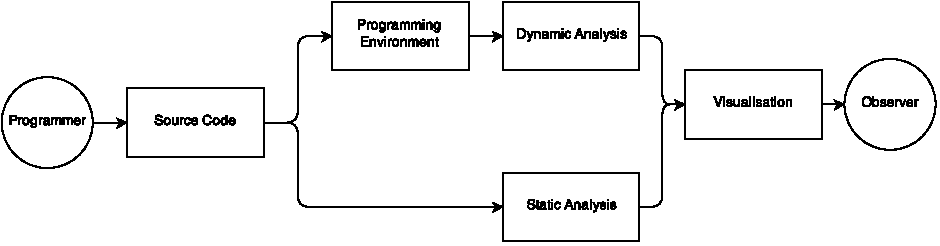
\includegraphics[width=\columnwidth]{../images/diagrams/knowledge-flow-refined.pdf}
  \caption{Knowledge flow from programmer to observer as directed by the visualisation technique employed.}
\label{fig:knowledge-flow-refined}
\end{figure}

\begin{figure}
  \centering 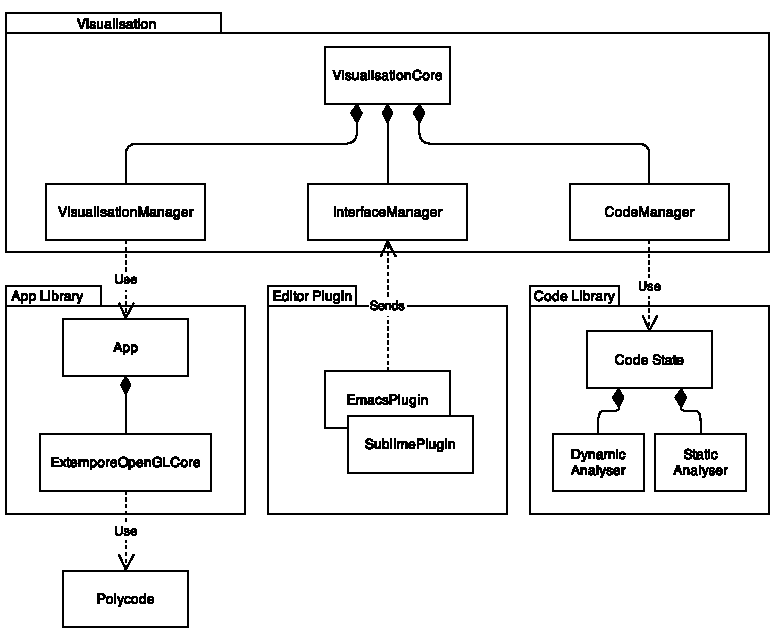
\includegraphics[width=\columnwidth]{../images/diagrams/visualisation-class-diagram.pdf}
  \caption{Class diagram of the visualisation technique employed.}
\label{fig:visualisation-class-diagram}
\end{figure}

The visualisation technique employed required three major components including an application manager, a code manager and an editor plugin (see the class diagram in Figure~\ref{fig:visualisation-class-diagram}). The following sections detail the implementation of these components.

\subsection{Application Manager}

-polycode~\cite{Safrin2013}

-opengl

\subsection{Code Manager}

-static analysis

-dynamic analysis

\subsection{Editor Plugin}

-sublime plugin

-emacs plugin

\section{Analysis}

Both dynamic program analysis and static source code analysis have been used to implement the visualisations (see combined static and dynamic approach taken in \cite{Eisenbarth2003})....

\section{Mappings}

A number of specific mappings were assigned to the visualisation. These visual mappings related directly to actions taken by the programmer. 

% See Table~\ref{} for a listing of these mappings.

